\documentclass{vkr}
\usepackage[english, russian]{babel} % переносы
\usepackage{graphicx} % для вставки картинок
\graphicspath{{images/}} % путь к изображениям
\usepackage[hidelinks]{hyperref}
\usepackage{float} % определяет метод H для рисунка с переносом на следующую страницу, ели не помещается
\usepackage{pdflscape}
\addto{\captionsrussian}{\renewcommand{\refname}{СПИСОК ИСПОЛЬЗОВАННЫХ ИСТОЧНИКОВ}}
\usepackage{xltabular} % для вставки таблиц
\usepackage{makecell}
\renewcommand\theadfont{} % шрифт в /thead
\usepackage{array} % для определения новых типов столбцов таблиц
\newcolumntype{T}{>{\centering\arraybackslash}X} % новый тип столбца T - автоматическая ширина столбца с выравниванием по центру
\newcolumntype{R}{>{\raggedleft\arraybackslash}X} % новый тип столбца R - автоматическая ширина столбца с выравниванием по правому краю
\newcolumntype{C}[1]{>{\centering\let\newline\\\arraybackslash\hspace{0pt}}m{#1}} % новый тип столбца C - фиксированная ширина столбца с выравниванием по центру
\newcolumntype{r}[1]{>{\raggedleft\arraybackslash}p{#1}} % новый тип столбца r - фиксированная ширина столбца с выравниванием по правому краю
\newcommand{\centrow}{\centering\arraybackslash} % командой \centrow можно центрировать одну ячейку (заголовок) в столбце типа X или p, оставив в оcтальных ячейках другой тип выравнивания
\newcommand{\finishhead}{\endhead\hline\endlastfoot}
\newcommand{\continuecaption}[1]{\captionsetup{labelformat=empty} \caption[]{#1}\\ \hline }
\usepackage{etoolbox}
\AtBeginEnvironment{xltabular}{\refstepcounter{tablecnt}} % подсчет таблиц xltabular, обычные таблицы подсчитываются в классе

\usepackage[tableposition=top]{caption} % подпись таблицы вверху
\captionsetup{strut=off}
\setlength{\intextsep}{0pt} % Vertical space above & below [h] floats
\setlength{\textfloatsep}{0pt} % Vertical space below (above) [t] ([b]) floats
\DeclareCaptionLabelFormat{gostfigure}{Рисунок #2} %подпись рисунка
\DeclareCaptionLabelFormat{gosttable}{Таблица #2} %подпись таблицы
\DeclareCaptionLabelSeparator{gost}{~--~} %разделитель в рисунках и таблицах
\captionsetup{labelsep=gost}
\captionsetup[figure]{aboveskip=10pt,belowskip=4mm,justification=centering,labelformat=gostfigure} % настройка подписи рисунка
\captionsetup[table]{font={stretch=1.41},skip=0pt,belowskip=0pt,aboveskip=8.5pt,singlelinecheck=off,labelformat=gosttable} % настройка подписи таблицы

\setlength{\LTpre}{8mm} % отступ сверху таблицы
\setlength{\LTpost}{6mm} % отступ снизу таблицы

\usepackage{enumitem}
\setlist{nolistsep,wide=\parindent,itemindent=*} % отступы вокруг списков, выравнивание с учетом разделителя

\usepackage{color} %% это для отображения цвета в коде
\usepackage{listings} %% листинги кода
\setmonofont[Scale=0.7]{Verdana} % моноширный шрифт для листинга

\definecolor{codegreen}{rgb}{0,0.6,0}
\definecolor{codegray}{rgb}{0.5,0.5,0.5}
\definecolor{codepurple}{rgb}{0.58,0,0.82}

\lstset{ %
language=C,                 % выбор языка для подсветки (здесь это С)
numbers=left,               % где поставить нумерацию строк (слева\справа)
numberstyle=\tiny,           % размер шрифта для номеров строк
stepnumber=1,                   % размер шага между двумя номерами строк
numbersep=5pt,                % как далеко отстоят номера строк от подсвечиваемого кода
commentstyle=\color{codegreen},
keywordstyle=\color{magenta},
numberstyle=\tiny\color{codegray},
stringstyle=\color{codepurple},
basicstyle=\linespread{0.95}\ttfamily,
backgroundcolor=\color{white}, % цвет фона подсветки - используем \usepackage{color}
showspaces=false,            % показывать или нет пробелы специальными отступами
showstringspaces=false,      % показывать или нет пробелы в строках
showtabs=false,             % показывать или нет табуляцию в строках
frame=single,              % рисовать рамку вокруг кода
tabsize=2,                 % размер табуляции по умолчанию равен 2 пробелам
captionpos=t,              % позиция заголовка вверху [t] или внизу [b] 
breaklines=true,           % автоматически переносить строки (да\нет)
breakatwhitespace=false, % переносить строки только если есть пробел
escapeinside={\%*}{*)}   % если нужно добавить комментарии в коде
}

\makeatletter % чтобы допускались русские комментарии в листингах
\lst@InputCatcodes
\def\lst@DefEC{%
 \lst@CCECUse \lst@ProcessLetter
  ^^80^^81^^82^^83^^84^^85^^86^^87^^88^^89^^8a^^8b^^8c^^8d^^8e^^8f%
  ^^90^^91^^92^^93^^94^^95^^96^^97^^98^^99^^9a^^9b^^9c^^9d^^9e^^9f%
  ^^a0^^a1^^a2^^a3^^a4^^a5^^a6^^a7^^a8^^a9^^aa^^ab^^ac^^ad^^ae^^af%
  ^^b0^^b1^^b2^^b3^^b4^^b5^^b6^^b7^^b8^^b9^^ba^^bb^^bc^^bd^^be^^bf%
  ^^c0^^c1^^c2^^c3^^c4^^c5^^c6^^c7^^c8^^c9^^ca^^cb^^cc^^cd^^ce^^cf%
  ^^d0^^d1^^d2^^d3^^d4^^d5^^d6^^d7^^d8^^d9^^da^^db^^dc^^dd^^de^^df%
  ^^e0^^e1^^e2^^e3^^e4^^e5^^e6^^e7^^e8^^e9^^ea^^eb^^ec^^ed^^ee^^ef%
  ^^f0^^f1^^f2^^f3^^f4^^f5^^f6^^f7^^f8^^f9^^fa^^fb^^fc^^fd^^fe^^ff%
  ^^^^20ac^^^^0153^^^^0152%
  % Basic Cyrillic alphabet coverage
  ^^^^0410^^^^0411^^^^0412^^^^0413^^^^0414^^^^0415^^^^0416^^^^0417%
  ^^^^0418^^^^0419^^^^041a^^^^041b^^^^041c^^^^041d^^^^041e^^^^041f%
  ^^^^0420^^^^0421^^^^0422^^^^0423^^^^0424^^^^0425^^^^0426^^^^0427%
  ^^^^0428^^^^0429^^^^042a^^^^042b^^^^042c^^^^042d^^^^042e^^^^042f%
  ^^^^0430^^^^0431^^^^0432^^^^0433^^^^0434^^^^0435^^^^0436^^^^0437%
  ^^^^0438^^^^0439^^^^043a^^^^043b^^^^043c^^^^043d^^^^043e^^^^043f%
  ^^^^0440^^^^0441^^^^0442^^^^0443^^^^0444^^^^0445^^^^0446^^^^0447%
  ^^^^0448^^^^0449^^^^044a^^^^044b^^^^044c^^^^044d^^^^044e^^^^044f%
  ^^^^0401^^^^0451%
  %%%
  ^^00}
\lst@RestoreCatcodes
\makeatother


% Режим шаблона (должен быть включен один из трех)
%\ВКРtrue
\Практикаtrue
%\Курсоваяtrue

\newcommand{\Дисциплина}{<<Проектирование и архитектура программных систем>>} % для курсовой
\newcommand{\КодСпециальности}{09.03.04} % Курсовая
\newcommand{\Специальность}{Программная инженерия} % Курсовая
\newcommand{\Тема}{Разработка web-сайта «Русатом – Аддитивные технологии» на платформе} % ВКР Курсовая
\newcommand{\ТемаВтораяСтрока}{1С-Битрикс}
\newcommand{\ГдеПроводитсяПрактика}{ООО "Предприятие ВТИ-Сервис"} % для практики
\newcommand{\РуководительПрактПредпр}{Федосов Д. В.} % для практики
\newcommand{\ДолжнРуководительПрактПредпр}{директор} % для практики
\newcommand{\РуководительПрактУнивер}{Чаплыгин А. А.} % для практики
\newcommand{\ДолжнРуководительПрактУнивер}{к.т.н. доцент} % для практики
\newcommand{\Автор}{В. Е. Зеленцов}
\newcommand{\АвторРод}{Зеленцова В. Е.}
\newcommand{\АвторПолностьюРод}{Зеленцова Виталия Евгеньевича} % для практики
\newcommand{\Шифр}{20-06-0045}
\newcommand{\Курс}{4} % для практики
\newcommand{\Группа}{ПО-01б}
\newcommand{\Руководитель}{А. А. Чаплыгин} % для ВКР и курсовой
\newcommand{\Нормоконтроль}{А. А. Чаплыгин} % для ВКР
\newcommand{\ЗавКаф}{А. В. Малышев} % для ВКР
\newcommand{\ДатаПриказа}{«07» апреля 2023~г.} % для ВКР
\newcommand{\НомерПриказа}{1505-с} % для ВКР
\newcommand{\СрокПредоставления}{«13» июня 2023~г.} % для ВКР, курсового

\begin{document}
\maketitle
\ifПрактика{}\else{
   \newpage
\begin{center}
\large\textbf{Минобрнауки России}

\large\textbf{Юго-Западный государственный университет}
\vskip 1em
\normalsize{Кафедра программной инженерии}
\vskip 1em
\ifВКР{
        \begin{flushright}
        \begin{tabular}{p{.4\textwidth}}
        \centrow УТВЕРЖДАЮ: \\
        \centrow Заведующий кафедрой \\
        \hrulefill \\
        \setarstrut{\footnotesize}
        \centrow\footnotesize{(подпись, инициалы, фамилия)}\\
        \restorearstrut
        «\underline{\hspace{1cm}}»
        \underline{\hspace{3cm}}
        20\underline{\hspace{1cm}} г.\\
        \end{tabular}
        \end{flushright}
        }\fi
\end{center}
\vspace{1em}
  \begin{center}
  \large
\ifВКР{
ЗАДАНИЕ НА ВЫПУСКНУЮ КВАЛИФИКАЦИОННУЮ РАБОТУ
  ПО ПРОГРАММЕ БАКАЛАВРИАТА}
  \else
ЗАДАНИЕ НА КУРСОВУЮ РАБОТУ (ПРОЕКТ)
\fi
\normalsize
  \end{center}
\vspace{1em}
{\parindent0pt
  Студента \АвторРод, шифр\ \Шифр, группа \Группа
  
1. Тема «\Тема\ \ТемаВтораяСтрока»
\ifВКР{
утверждена приказом ректора ЮЗГУ от \ДатаПриказа\ № \НомерПриказа
}\fi.

2. Срок предоставления работы к защите \СрокПредоставления

3. Исходные данные для создания программной системы:

3.1. Перечень решаемых задач:}

\renewcommand\labelenumi{\theenumi)}

\begin{enumerate}
\item проанализировать IT-инфраструктуру предприятия;
\item  разработать концептуальную модель системы управления IT-ин\-фра\-струк\-турой предприятия на основе подхода к управлению и организации ИТ-услуг ITSM;
\item спроектировать программную систему управления IT-ин\-фра\-струк\-турой предприятия;
\item сконструировать и протестировать программную систему управления IT-инфраструктурой предприятия.
\end{enumerate}

{\parindent0pt
  3.2. Входные данные и требуемые результаты для программы:}

\begin{enumerate}
\item Входными данными для программной системы являются: данные
справочников комплектующих, конфигураций, ПО, критериев качества SLA,
ИТ-услуг, департаментов компании; технические данные ИТ-ресурсов; данные входящих заявок на ИТ-ресурсы; данные запросов поставщикам на комплектующие.
\item Выходными данными для программной системы являются: сформированные заявки на обслуживание ИТ-ресурсов; сформированные запросы на
закупку комплектующих; сведения о выполненных работах по заявкам; статусы заявок; выходные отчеты (инфографика) – по качеству услуг, по состоянию ИТ-ресурсов, по деятельности ИТ-отдела, по стоимости обслуживания
ИТ-ресурсов, воронка заявок.
\end{enumerate}

{\parindent0pt

  4. Содержание работы (по разделам):
  
  4.1. Введение
  
  4.1. Анализ предметной области
  
4.2. Техническое задание: основание для разработки, назначение разработки,
требования к программной системе, требования к оформлению документации.

4.3. Технический проект: общие сведения о программной системе, проект
данных программной системы, проектирование архитектуры программной системы, проектирование пользовательского интерфейса программной системы.

4.4. Рабочий проект: спецификация компонентов и классов программной системы, тестирование программной системы, сборка компонентов программной системы.

4.5. Заключение

4.6. Список использованных источников

5. Перечень графического материала:

\списокПлакатов

\vskip 2em
\begin{tabular}{p{6.8cm}C{3.8cm}C{4.8cm}}
Руководитель \ifВКР{ВКР}\else работы (проекта) \fi & \lhrulefill{\fill} & \fillcenter\Руководитель\\
\setarstrut{\footnotesize}
& \footnotesize{(подпись, дата)} & \footnotesize{(инициалы, фамилия)}\\
\restorearstrut
Задание принял к исполнению & \lhrulefill{\fill} & \fillcenter\Автор\\
\setarstrut{\footnotesize}
& \footnotesize{(подпись, дата)} & \footnotesize{(инициалы, фамилия)}\\
\restorearstrut
\end{tabular}
}

\renewcommand\labelenumi{\theenumi.}

   \abstract{РЕФЕРАТ}

Объем работы равен \formbytotal{lastpage}{страниц}{е}{ам}{ам}. Работа содержит \formbytotal{figurecnt}{иллюстраци}{ю}{и}{й}, \formbytotal{tablecnt}{таблиц}{у}{ы}{}, \arabic{bibcount} библиографических источников и \formbytotal{числоПлакатов}{лист}{}{а}{ов} графического материала. Количество приложений – 2. Графический материал представлен в приложении А. Фрагменты исходного кода представлены в приложении Б.

Перечень ключевых слов: коммерческий сайт, Система, CMS, Битрикс, Joomla, аддитивные технологии, 3D-принтеры, услуги, сервисы, информатизация, автоматизация, информационные технологии, веб-форма,  Apache, классы, база данных, средства защиты информации, подсистема, компонент, модуль, сущность, информационный блок, метод, контент-редактор, администратор, пользователь, web-сайт.

Объектом разработки является web-сайт компании,  занимающейся производством 3D-принтеров, выпуском оборудования для создания порошков, разработкой программного обеспечения и организацией центров аддитивного производства.

Целью выпускной квалификационной работы является привлечение клиентов, увеличение заказов, информирование о продукции и услугах путем создания сайта компании.

В процессе создания сайта были выделены основные сущности путем создания информационных блоков, использованы классы и методы модулей, обеспечивающие работу с сущностями предметной области, а также корректную работу web-сайта, разработаны разделы, содержащие информацию о компании, ее деятельности, производимой продукции и услугах, разработан сервис по заказу 3D-деталей.

При разработке сайта использовалась система управления контентом "<1С-Битрикс: Управление сайтом">.

Разработанный сайт был успешно внедрен в компании.

\selectlanguage{english}
\abstract{ABSTRACT}
  
The volume of work is \formbytotal{lastpage}{page}{}{s}{s}. The work contains \formbytotal{figurecnt}{illustration}{}{s}{s}, \formbytotal{tablecnt}{table}{}{s}{s}, \arabic{bibcount} bibliographic sources and \formbytotal{числоПлакатов}{sheet}{}{s}{s} of graphic material. The number of applications is 2. The graphic material is presented in annex A. The layout of the site, including the connection of components, is presented in annex B.

List of keywords: commercial website, System, CMS, Bitrix, Joomla, additive technologies, 3D printers, services, services, informatization, automation, information technology, web form, Apache, classes, database, component, module, entity, information block, method, content editor, administrator, user, web site.

The object of the research is the analysis of information technologies for the development of a production company's website.

The object of the development is the website of a company engaged in the production of 3D printers, the production of equipment for the creation of powders, software development and the organization of additive manufacturing centers.

The purpose of the final qualifying work is to attract customers, increase orders, inform about products and services by creating a company website.

In the process of creating the site, the main entities were identified by creating information blocks, classes and methods of modules were used to ensure work with the entities of the subject area, as well as the correct operation of the website, sections containing information about the company, its activities, products and services were developed, a service for ordering 3D parts was developed.

When developing the site, the content management system <<1C – Bitrix: Site Management>> was used.

The developed website was successfully implemented in the company.
\selectlanguage{russian}
}\fi
\tableofcontents
\section*{ОБОЗНАЧЕНИЯ И СОКРАЩЕНИЯ}

БД -- база данных.

ИС -- информационная система.

ИТ -- информационные технологии. 

КТС -- комплекс технических средств.

ОМТС -- отдел материально-технического снабжения. 

ПО -- программное обеспечение.

РП -- рабочий проект.

СУБД -- система управления базами данных.

ТЗ -- техническое задание.

ТП -- технический проект.

UML (Unified Modelling Language) -- язык графического описания для объектного моделирования в области разработки программного обеспечения.

\ifПрактика{}\else{\section*{ВВЕДЕНИЕ}
\addcontentsline{toc}{section}{ВВЕДЕНИЕ}

Аддитивные технологии (АТ) начали активно развиваться со времени получения первых трехмерных изображений изделий на дисплеях компьютеров. Начало положила стереолитография, затем довольно многочисленные новые принципы стали называть технологиями быстрого прототипирования, затем укоренилось название "<Аддитивные технологии">. Интенсивность развития данных технологий не имеет аналогов. АТ изменили процессы проектирования и конструирования изделий, превратив их в процессы непрерывного создания изделий. Современные проектирование и производство изделий невозможно представить без данного рода технологий. 3D-принтеры стали такими же распространенными, как и персональные компьютеры. С помощью 3D-принтеров получают ткани, обувь, продукты питания, а также выращивают человеческие органы. Во многих отраслях, например, в космической отрасли, альтернативы аддитивным технологиям нет.

АТ предполагают изготовление детали методом послойного нанесения материала, в отличие от традиционных методов формирования детали, за счёт удаления материала из массива заготовки.

При использовании АТ все стадии реализации проекта от идеи до материализации находятся в единой технологической цепи, в которой каждая технологическая операция выполняется в цифровой CAD/CAM/CAE-системе.

Современные компании, видя, как развиваются информационные технологии, пытаются использовать их выгодно для своего бизнеса, поэтому запускают свой web-сайт. С его помощью предприятие может заявить о себе, проинформировать потенциального заказчика об услугах или продуктах, которые предоставляет, а также позволяет пользователям сделать с помощью сайта онлайн-заказ, произвести покупку или оплатить счета.

Сайт считается лицом компании и может существенно повысить ее имидж. Любой пользователь сети Интернет сможет получить необходимую информацию о компании в любой момент, появляется возможность найти контактные телефоны, адрес и e-mail, чтобы связаться с компанией. Сейчас большинство клиентов узнают о ее существовании именно через сайт. Поэтому сайт можно назвать самой лучшей рекламой. 

Главной задачей профессионально построенного сайта является превращение посетителя, зашедшего на сайт, в потенциального клиента.

\emph{Цель настоящей работы} – разработка web-сайта компании для привлечения новой аудитории, увеличения заказов, рекламы продукции и услуг компании. Для достижения поставленной цели необходимо решить \emph{следующие задачи:}
\begin{itemize}
\item провести анализ предметной области;
\item разработать концептуальную модель web-сайта;
\item спроектировать web-сайт;
\item реализовать сайт средствами web-технологий.
\end{itemize}

\emph{Структура и объем работы.} Отчет состоит из введения, 4 разделов основной части, заключения, списка использованных источников, 2 приложений. Текст выпускной квалификационной работы равен \formbytotal{page}{страниц}{е}{ам}{ам}.

\emph{Во введении} сформулирована цель работы, поставлены задачи разработки, описана структура работы, приведено краткое содержание каждого из разделов.

\emph{В первом разделе} на стадии описания технической характеристики предметной области приводится сбор информации о деятельности компании, для которой осуществляется разработка сайта.

\emph{Во втором разделе} на стадии технического задания приводятся требования к разрабатываемому сайту.

\emph{В третьем разделе} на стадии технического проектирования представлены проектные решения для web-сайта.

\emph{В четвертом разделе} приводится список классов и их методов, использованных при разработке сайта, производится тестирование разработанного сайта.

В заключении излагаются основные результаты работы, полученные в ходе разработки.

В приложении А представлен графический материал.
В приложении Б представлены фрагменты исходного кода. 
}\fi
\section{Анализ предметной области}
\subsection{Сервисы для обмена и продажи виртуальных ценностей в MMORPG}

В мире массовых многопользовательских онлайн-игр (MMORPG), таких как «Stay Out», игроки могут взаимодействовать в виртуальном мире, выполнять квесты, сражаться с монстрами, развивать своих персонажей и, конечно же, торговать внутриигровыми ценностями. MMORPG представляют собой уникальный игровой жанр, где тысячи игроков со всего мира могут взаимодействовать между собой в одном виртуальном мире, создавая атмосферу постоянного развития и приключений.

Сервисы для обмена и продажи виртуальных ценностей в MMORPG призван упростить процесс торговли между игроками, предоставляя им удобную платформу для взаимодействия. Необходимость в таком сервисе возникает из-за того, что в некоторых играх обмен виртуальными ценностями может быть неудобным и невыгодным для игроков. Это может приводить к созданию различных групп в социальных сетях и мессенджерах, где игроки выкладывают свои товары и договариваются о сделках.

Целью таких сервисов является упрощение процесса торговли, делая его более удобным и безопасным для всех участников. Путем создания специализированной платформы для обмена и продажи виртуальных ценностей, игрокам будет легче находить нужные товары, договариваться о цене и завершать сделки, минимизируя риск обмана и недобросовестных сделок.

Преимущества сервиса для обмена виртуальными ценностями:
\begin{itemize}
	\item Экономия ресурсов: Сервис не требует значительных ресурсов для использования и позволяет игрокам свободно обмениваться своими предметами.
	\item Удобство взаимодействия: Пользователи могут легко связываться друг с другом, договариваться о цене и условиях сделки, что делает процесс торговли более удобным и эффективным.
	\item Минимизация рисков обмана: В отличие от торговли в группах в социальных сетях, где информация о товарах может быть неполной или недостоверной, сервис предоставляет полные характеристики предметов с самого начала сделки, что уменьшает риск обмана.
	\item Отсутствие вмешательства администрации: В сервисах для обмена виртуальными ценностями нет лишней административной информации и правил, устанавливаемых владельцем группы или сообщества, что делает процесс торговли более прозрачным и справедливым для всех участников.
	\item Быстрый поиск товаров: Пользователи могут легко найти необходимый товар и просмотреть все предложения на рынке в считанные секунды благодаря удобному интерфейсу и системе поиска.
\end{itemize}
\subsection{Характеристика игры "<Stay Out">}

"<Stay Out"> представляет собой онлайн-игру в жанре выживания и RPG, где игроки исследуют постапокалиптический мир, выполняют различные задания и сражаются с мутантами. Для выставления товара на продажу в игре требуется уплата комиссии в размере 4\%, а сами предметы могут достигать высоких цен в 1 миллиард, что делает данный процент неоправданно высоким. Кроме того, товары выставляются временно, всего на 2 дня, после чего возвращаются на склад, а комиссия за торговлю исчезает. Поиск товаров в игре осуществляется дословно, что затрудняет процесс поиска нужных предметов.

\section{Техническое задание}
\subsection{Основание для разработки}

Основанием для разработки является задание на выпускную квалификационную работу бакалавра "<Маркетплейс для реализации цифровых предметов внутри игры \textquotedbl Stay Out\textquotedbl">.

\subsection{Цель и назначение разработки}

Основной задачей выпускной квалификационной работы является разработка и внедрение web-сайта для упрощения торговли внутриигровыми ценностями в «Stay Out».


В процессе разработки web-сайта для упрощения торговли внутриигровыми ценностями в «Stay Out» можно выделить следующие задачи:
\begin{itemize}
\item реализация системы аутентификации и безопасности;
\item разработка функционала поиска и фильтрации товаров;
\item внедрение системы обратной связи;
\item разработка системы управления контентом;
\item внедрение механизмов модерации.
\end{itemize}

\subsection{Требования пользователя к интерфейсу web-сайта}

Сайт должен включать в себя:
\begin{itemize}
    \item поиск предметов;
    \item авторизацию;
    \item регистрацию;
    \item выбор сервера;
    \item доступ к профилю.
\end{itemize}

Композиция шаблона сайта представлена на рисунке ~\ref{fig:image}.
\begin{figure}[ht]
	\centering
	
\includegraphics[width=1\linewidth]{images/image}
	\caption{Композиция шаблона сайта}
	\label{fig:image}
\end{figure}
%\vspace{-\figureaboveskip} % двойной отступ не нужен (можно использовать, если раздел заканчивается картинкой)

\subsection{Функциональные требования к программной системе}

Для разрабатываемого сайта была реализована модель, которая обеспечивает наглядное представление вариантов использования сайта.

Она помогает в физической разработке и детальном анализе взаимосвязей объектов. При построении диаграммы вариантов использования применяется унифицированный язык визуального моделирования UML.

Диаграмма вариантов описывает функциональное назначение разрабатываемой системы. То есть это то, что система будет непосредственно делать в процессе своего функционирования. Она является исходным концептуальным представлением системы в процессе ее проектирования и разработки. Проектируемая система представляется в виде ряда прецедентов, предоставляемых системой актерам или сущностям, которые взаимодействуют с системой. Актером или действующим лицом является сущность, взаимодействующая с системой извне (например, человек, техническое устройство). Прецедент служит для описания набора действий, которые система предоставляет актеру.

На основании анализа предметной области в разрабатываемой программно-информационной системе должны быть реализованы следующие функции:
\begin{enumerate}
\item Регистрация нового пользователя.
\item Вход пользователя в систему.
\item Просмотр списка выставленных предметов.
\item Поиск предметов.
\item Просмотр подробной информации о товаре.
\item Выставление предмета на продажу/покупку.
\item Управление личным профилем.
\item Отправка сообщений другим пользователям.
\item Получение сообщений от других пользователей.
\end{enumerate}

На рисунке ~\ref{fig:-} в виде диаграммы прецедентов представлены функциональные требования к системе для пользователей.

\begin{figure}[th]
	\centering
	\includegraphics[width=1\linewidth]{"images/Диаграмма прецедентов"}
	\caption{Диаграмма прецедентов}
	\label{fig:-}
\end{figure}

\subsubsection{Вариант использования «Выбор сервера»}

Заинтересованные лица и их требования: пользователь желает начать производить какие-либо действия на сайте, связанные с торговлей.
Предусловие: открыта главная страница сайта.
Постусловие: открывается нужная страница в соответствие с выбранным сервером.
Основной успешный сценарий:
\begin{enumerate}
	\item Пользователь нажимает на кнопку выбора сервера на главной странице сайта.
	\item На сайте открывается модальное окно с доступными серверами.
	\item Пользователь выбирает нужный ему сервер.
	\item Приложение открывает страницу, соответствующую выбранному серверу
\end{enumerate}

\subsubsection{Вариант использования «Смена сервера»}

Заинтересованные лица и их требования: пользователь играет сразу на нескольких серверах и хочет выполнить какие-либо действия, связанные с торговлей, на другом сервере.
Предусловие: открыта страница какого-либо сервера.
Постусловие: открывается нужная страница в соответствие с выбранным сервером.
Основной успешный сценарий:
\begin{enumerate}
	\item Пользователь нажимает на кнопку «Сменить сервер».
	\item На сайте открывается модальное окно с другими серверами.
	\item Пользователь выбирает нужный ему сервер.
	\item Приложение открывает страницу, соответствующую выбранному серверу
\end{enumerate}

\subsubsection{Вариант использования «Поиск»}

Заинтересованные лица и их требования: пользователь желает произвести поиск товаров, имеющих в названии одно или несколько ключевых слов.
Предусловие: открыта страница какого-либо сервера.
Постусловие: лента перезагружается, при наличии товаров, соответствующих поисковому запросу в базе данных, будет отображен их список.
Если товары отсутствуют, отображается пустой список.
Основной успешный сценарий:
\begin{enumerate}
	\item Пользователь переходит в режим поиска путем нажатия на элемент интерфейса (значок с изображением лупы) и ввода поискового запроса.
	\item Приложение передает поисковой запрос на сервер.
	\item Сервер формирует запрос в базу данных и передает результат в приложение.
	\item Приложение получает информацию от сервера и производит модификацию списка отображаемых товаров.
\end{enumerate}

\subsubsection{Вариант использования «Просмотр информации о товаре»}

Заинтересованные лица и их требования: пользователь желает получить больше информации о конкретном товаре.
Предусловие: открыта страница какого-либо сервера.
Постусловие: появляется модальное окно с полной информацией о товаре.
Основной успешный сценарий:
\begin{enumerate}
	\item Пользователь нажимает на значок с изображением нужного товара.
	\item Приложение получает уникальный id предмета и отправляет запрос на сервер.
	\item Сервер формирует запрос в базу данных и передает данные в приложение.
	\item Приложение получает информацию от сервера и заполняет модальное окно в соответствие с полученной информацией.
\end{enumerate}

\subsubsection{Вариант использования «Покупка товара»}

Заинтересованные лица и их требования: пользователь увидел интересующий его товар и захотел его приобрести.
Предусловие: открыта страница какого-либо сервер.
Постусловие: появляется уникальное сообщение, которое нужно скопировать и вставить в игре.
Основной успешный сценарий:
\begin{enumerate}
	\item Пользователь нажимает на кнопку «Купить».
	\item Приложение генерирует уникальное сообщение в соответствие с названием товаров и игровым никнеймом пользователя.
\end{enumerate}

\subsubsection{Вариант использования «Регистрация»}

Заинтересованные лица и их требования: пользователь хочет создать свой аккаунт на сайте.
Предусловие: пользователь еще не авторизовался на сайте.
Постусловие: регистрация произведена, появляется значек с изображение профиля.
Основной успешный сценарий:
\begin{enumerate}
	\item Пользователь нажимает на кнопку «Регистрация».
	\item Открывается экран регистрации пользователя.
	\item Пользователь вводит почту, логин, пароль и повторный пароль.
	\item Приложение отправляет запрос на сервер.
	\item Сервер формирует запрос в базу данных на создание аккаунта.
	\item Если аккаунта с таким же логином или почтой не существует, создается новый аккаунт.
	\item Сервер передает информацию в приложение о результате создания аккаунта.
	\item Приложение открывает окно пользователю с результатами регистрации.
\end{enumerate}

\subsubsection{Вариант использования «Авторизация»}

Заинтересованные лица и их требования: пользователь хочет войти в свой аккаунт на сайте.
Предусловие: пользователь еще не авторизовался на сайте.
Постусловие: авторизация произведена, появляется значок с изображение профиля.
Основной успешный сценарий:
\begin{enumerate}
	\item Пользователь нажимает на кнопку «Авторизация».
	\item Открывается экран регистрации пользователя.
	\item Пользователь вводит почту, логин, пароль и повторный пароль.
	\item Приложение отправляет запрос на сервер.
	\item Сервер формирует запрос в базу данных на создание аккаунта.
	\item Если аккаунта с таким же логином или почтой не существует, создается новый аккаунт.
	\item Сервер передает информацию в приложение о результате создания аккаунта.
	\item Приложение открывает окно пользователю с результатами регистрации.
\end{enumerate}

\subsubsection{Вариант использования «Выставление товара»}

Заинтересованные лица и их требования: пользователь хочет продать какую-либо вещь.
Предусловие: пользователь выбрал сервер и авторизовался.
Постусловие: предмет добавляется в ленту товаров:
\begin{enumerate}
	\item Пользователь нажимает на элемент интерфейса (значок с изображением плюса).
	\item Приложение открывает модальное окно с полями ввода.
	\item Пользователь вводит название предмета полностью или его часть.
	\item Приложение выводит все совпадения.
	\item Пользователь выбирает нужный ему предмет.
	\item Приложение отправляет запрос на сервер.
	\item Сервер формирует запрос в базу данных на получения все характеристик предмета.
	\item Сервер передает данные в приложение.
	\item Приложение заполняет необходимые данные в соответствие с данными.
	\item Пользователь вводит недостающие данные и выставляет предмет на продажу.
	\item Приложение отправляет запрос на сервер.
	\item Сервер вносит данные в базу данных.
	\item Сервер передает информацию о результате приложению.
	\item Приложение оповещает пользователя об успехе выставления предмета на продажу
\end{enumerate}

\subsection{Требования к оформлению документации}

Разработка программной документации и программного изделия должна производиться согласно ГОСТ 19.102-77 и ГОСТ 34.601-90. Единая система программной документации.

\section{Технический проект}
\subsection{Общая характеристика организации решения задачи}

Необходимо разработать веб-платформу, специально адаптированную для упрощения процесса обмена внутриигровыми ценностями в игре "Stay Out".

Веб-сайт представляет собой комплекс электронных страниц, объединенных в логическую структуру и содержащих разнообразную информацию, включая текст, графику и мультимедийные элементы. Этот онлайн-ресурс доступен через Интернет по определенному доменному имени, например, www.stayoutexchange.com. Каждая страница веб-сайта представляет собой HTML-документ, который обеспечивает визуальное и функциональное взаимодействие с пользователем при помощи языков программирования, таких как HTML, CSS и JavaScript.

Разрабатываемый веб-сайт будет предоставлять пользователям возможность создания учетных записей, выставления и поиска внутриигровых ценностей, а также обмена ими с другими игроками. Он будет обеспечивать удобный интерфейс для взаимодействия между игроками, обеспечивая прозрачность и безопасность сделок.

\subsection{Обоснование выбора технологии проектирования}

Используемые для создания программно-информационной системы языки и технологии отвечают современным практикам разработки, позволяют достичь высокой производительности и отказоустойчивости программы.

\subsubsection{Описание используемых технологий и языков программирования}

В процессе разработки web-сайта используются программные средства и языки программирования. Каждое программное средство и каждый язык программирования применяется для круга задач, при решении которых они необходимы.

\subsubsection{Язык программирования JavaScript}

JavaScript - это интерпретируемый, объектно-ориентированный язык программирования, который широко используется для создания интерактивных и динамических веб-сайтов. Благодаря своей многофункциональности, JavaScript является одним из самых популярных языков программирования в мире веб-разработки.

В отличие от многих других языков программирования, JavaScript выполняется непосредственно в web-браузере пользователя. Это позволяет ему взаимодействовать с элементами HTML страницы, управлять их содержимым, изменять стили, реагировать на пользовательские действия и многое другое, что делает веб-страницы более интерактивными и динамичными.

JavaScript широко используется для разработки различных веб-приложений, таких как интерфейсы пользователя, игры, анимации, формы обратной связи, веб-сервисы и многое другое. Благодаря своей популярности и гибкости, JavaScript также стал широко используемым для разработки серверной стороны приложений с использованием платформы Node.js.

Язык JavaScript имеет динамическую типизацию данных, что означает, что переменные не требуют явного объявления типа данных, и их тип может изменяться в процессе выполнения программы. Это делает JavaScript гибким и удобным для быстрой разработки прототипов и простых скриптов.

Важно отметить, что JavaScript не следует путать с языком Java, несмотря на сходство в названиях. JavaScript и Java - это разные языки программирования с разными синтаксисами, целями и областями применения. JavaScript был создан компанией Netscape в начале 1990-х годов и был изначально разработан для управления взаимодействием с пользователем на веб-страницах.

\paragraph{Достоинства языка JavaScript}

JavaScript чаще всего используется для написания сценариев работы с web-страницами в web-браузерах, обеспечивая программирование на стороне клиента. Этот язык предоставляет возможность доступа к элементам разметки web-страницы посредством объектов, что значительно упрощает манипуляции с разметкой. Для решения сложностей с интерпретацией кода различными браузерами применяется библиотека jQuery, которая расширяет возможности JavaScript и унифицирует поведение кода между разными средами.

\paragraph{Недостатки языка Javascript}

JavaScript обладает некоторыми особенностями, например, непредсказуемость операций сравнения типов данных, что может привести к неожиданным результатам при выполнении математических операций или сравнении значений. Это создает потенциальные сложности для разработчиков, так как различные web-браузеры могут по-разному интерпретировать сценарии JavaScript. Неверно написанный код JavaScript может привести к труднообнаруживаемым ошибкам, и их отладка может быть затруднительной из-за специфики языка.

\subsection{Диаграмма компонентов и схема обмена данными между файлами компонента}

Диаграмма компонентов является важным инструментом для описания физического представления разрабатываемой системы. Она позволяет разработчикам определить архитектуру системы, выявив взаимосвязи и зависимости между программными компонентами, включая как исходный, так и исполняемый код.

Основными элементами диаграммы компонентов являются компоненты, интерфейсы и зависимости между ними. Компоненты представляют собой логические единицы функциональности системы, которые могут быть как отдельными приложениями, так и более крупными модулями или сервисами.

Интерфейсы определяют способы взаимодействия между компонентами, задавая набор методов, сообщений или протоколов, которыми компоненты обмениваются информацией.

Зависимости указывают на связи между компонентами, определяя порядок и направление потока данных или контроля между ними.

На рисунке \ref{fig:comp} представлена диаграмма компонентов для проектируемой системы. В центре диаграммы находится сервер с операционной системой, на которой установлена система управления содержимым. Эта система включает в себя базу данных и интерфейс для взаимодействия с клиентскими приложениями.

Помимо этого на диаграмме изображен клиентский компьютер с операционной системой, на которой установлен браузер. Этот компьютер предоставляет интерфейс для взаимодействия пользователя с системой через web-интерфейс.

\vspace{-8mm}
\begin{figure}
	\centering
	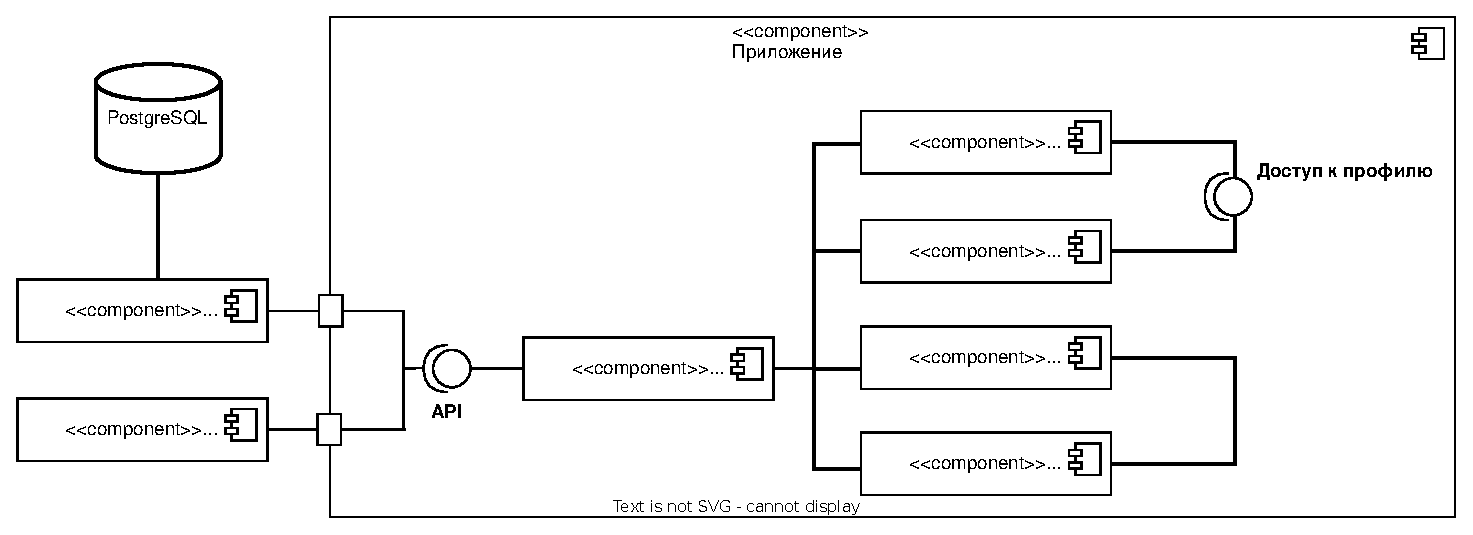
\includegraphics[width=1\linewidth]{images/comp}
	\caption{Диаграмма компонентов}
	\label{fig:comp}
\end{figure}

Любой компонент должен быть вызван в сценарии страницы web-сайта. Web-страница передает данные компоненту в момент вызова последнего.

При вызове компонента в сценарии web-страницы передаются значения параметров компонента, которые далее передаются в сценарий файла component.php через массив \$arParams.

В сценарии файла component.php происходит вызов одного из шаблонов компонента с помощью метода IncludeComponentTemplate класса CBitrixComponent. Id шаблона также определяется в сценарии страницы web-приложения и передается неявно методом IncludeComponentTemplate.

После вызова шаблона компонента, в файл template.php передается массив \$arParams, возможно, измененный в сценарии component.php, а также массив \$arResult, сформированный в самом сценарии component.php. Оба этих массива доступны также и в файле result\_modifier.php, который подключается перед template.php.

Работа компонента завершается после выполнения сценария файла component.php. Однако, если массив \$arResult будет изменен в сценарии шаблона, изменения не будут переданы обратно в сценарий файла компонента component.php.

\subsection{Диаграмма размещения}

Диаграмма размещения (рис.~\ref{fig:razm}) отражает физические взаимосвязи между программными и аппаратными компонентами системы.

\vspace{-8mm} % чтобы убрать пустую строку, которая осталась после переноса рисунка на следующую страницу
\begin{figure}
	\centering
	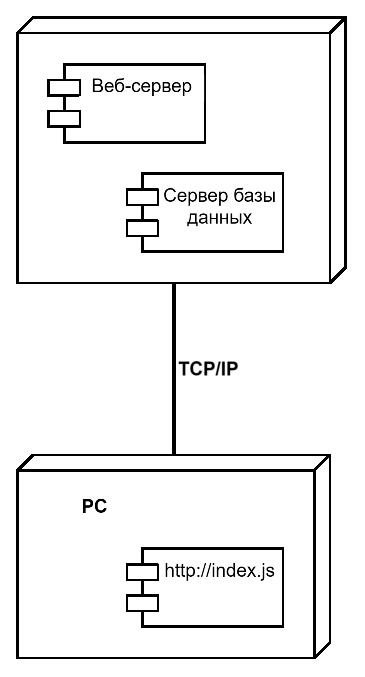
\includegraphics[width=0.5\linewidth]{images/razm}
	\caption{Диаграмма размещения}
	\label{fig:razm}
\end{figure}

Она является хорошим средством для показа маршрутов перемещения объектов и компонентов в распределенной системе.

В таблице \ref{ssevsws:table} приведен пример использования пакета xltabular с автоматическим расчетом ширины столбца.

\begin{xltabular}{\textwidth}{|c|X|X|}
	\caption{Сравнение протоколов SSE и WebSocket\label{ssevsws:table}}\\ \hline
	~  & \centrow  SSE & \centrow WebSocket \\ \hline
	\endfirsthead
	\continuecaption{Продолжение таблицы \ref{ssevsws:table}}
	~ & \centrow SSE & \centrow WebSocket \\ \hline 
	\finishhead
	Направленность & 
	Однонаправленный, полудуплексный: данные посылает только сервер & 
	Двунаправленный, полнодуплексный: и сервер, и клиент могут обмениваться сообщениями \\ \hline 
	Соединение  & HTTP & WS \\ \hline 
	Тип данных & Только текст & Бинарные и текстовые данные \\ \hline 
	Доп. возможности & Встроенный механизм идентификаторов событий и переподключения & Переподключение и идентификация события реализуются на стороне приложения
\end{xltabular}

\subsection{Содержание информационных блоков. Основные сущности}

Проанализировав требования, можно выделить шесть основных сущностей:
\begin{itemize}
\item "<Пользователь">;
\item "<Предметы">;
\item "<Услуги">.
\end{itemize}

В состав сущности "<Пользователь"> можно включить атрибуты, представленные в таблице \ref{news:table}.

\begin{xltabular}{\textwidth}{|l|l|p{1.7cm}|X|}
	\caption{Атрибуты сущности "<Пользователь">\label{news:table}}\\ \hline
	\centrow Поле & \centrow Тип & \centrow Обяза\-тельное & \centrow Описание \\ \hline
	\thead{1} & \thead{2} & \centrow 3 & \centrow 4 \\ \hline
	\endfirsthead
	\continuecaption{Продолжение таблицы \ref{news:table}}
	\thead{1} & \thead{2} & \centrow 3 & \centrow 4 \\ \hline
	\finishhead
	id & ObjectId & true & Уникальный идентификатор \\ \hline 
	email & String & true & Почта \\ \hline 
	login & String & true & Псевдоним \\ \hline
	password & String & true & Пароль \\ \hline 
	role & String & true & Привилегия \\ \hline 
	status & String & true & Статус \\ \hline 
\end{xltabular}

В состав сущности "<Предметы"> можно включить атрибуты, представленные в таблице \ref{proda:table}.

\begin{xltabular}{\textwidth}{|R|C{2.5cm}|l|T|}
	\caption{Атрибуты  сущности "<Предметы"> с использованием различных типов столбцов и многострочным заголовком\label{proda:table}}\\ \hline
	\centrow Поле & \centrow Тип & \centrow Обязательное & \centrow Описание \\ \hline
	\centrow 1 & \centrow 2 & \thead{3} & \centrow 4 \\ \hline
	\endfirsthead
	\continuecaption{Продолжение таблицы \ref{proda:table}}
	\centrow 1 & \centrow 2 & \thead{3} & \centrow 4 \\ \hline
	\finishhead
	id & ObjectId & true & Уникальный идентификатор \\ \hline 
	name & String & true & Название \\ \hline 
	description & String & false & Описание \\ \hline 
	img & String & true & Путь до изображения \\ \hline 
	weight & String & true & Вес \\ \hline 
	level & String & true & Уровень \\ \hline 
\end{xltabular}

В состав сущности "<Тип"> можно включить атрибуты, представленные в таблице \ref{prod1:table}.

\begin{xltabular}{\textwidth}{|R|C{2.5cm}|l|T|}
	\caption{Атрибуты  сущности "<Тип"> с использованием различных типов столбцов и многострочным заголовком\label{prod1:table}}\\ \hline
	\centrow Поле & \centrow Тип & \centrow Обязательное & \centrow Описание \\ \hline
	\centrow 1 & \centrow 2 & \thead{3} & \centrow 4 \\ \hline
	\endfirsthead
	\continuecaption{Продолжение таблицы \ref{prod1:table}}
	\centrow 1 & \centrow 2 & \thead{3} & \centrow 4 \\ \hline
	\finishhead
	id & ObjectId & true & Уникальный идентификатор \\ \hline 
	name & String & true & Название \\ \hline 
	img & String & true & Путь до изображения \\ \hline 
\end{xltabular}

В состав сущности "<Класс"> можно включить атрибуты, представленные в таблице \ref{prod2:table}.

\begin{xltabular}{\textwidth}{|R|C{2.5cm}|l|T|}
	\caption{Атрибуты  сущности "<Класс"> с использованием различных типов столбцов и многострочным заголовком\label{prod2:table}}\\ \hline
	\centrow Поле & \centrow Тип & \centrow Обязательное & \centrow Описание \\ \hline
	\centrow 1 & \centrow 2 & \thead{3} & \centrow 4 \\ \hline
	\endfirsthead
	\continuecaption{Продолжение таблицы \ref{prod2:table}}
	\centrow 1 & \centrow 2 & \thead{3} & \centrow 4 \\ \hline
	\finishhead
	id & ObjectId & true & Уникальный идентификатор \\ \hline 
	name & String & true & Название \\ \hline 
	img & String & true & Путь до изображения \\ \hline 
\end{xltabular}

В состав сущности "<Экипировка"> можно включить атрибуты, представленные в таблице \ref{prod3:table}.

\begin{xltabular}{\textwidth}{|R|C{2.5cm}|l|T|}
	\caption{Атрибуты  сущности "<Экипировка"> с использованием различных типов столбцов и многострочным заголовком\label{prod3:table}}\\ \hline
	\centrow Поле & \centrow Тип & \centrow Обязательное & \centrow Описание \\ \hline
	\centrow 1 & \centrow 2 & \thead{3} & \centrow 4 \\ \hline
	\endfirsthead
	\continuecaption{Продолжение таблицы \ref{prod3:table}}
	\centrow 1 & \centrow 2 & \thead{3} & \centrow 4 \\ \hline
	\finishhead
	id & ObjectId & true & Уникальный идентификатор \\ \hline 
	lifting\_capacity & String & true & Грузоподъемность \\ \hline 
	melee & String & true & Рукопашная \\ \hline 
	explosion & String & true & Взрыв \\ \hline
	electric & String & true & Электрическое \\ \hline 
	infrared & String & true & Инфракрасное \\ \hline 
	radiation & String & true & Радиация \\ \hline 
	biological & String & true & Биологическое \\ \hline 
	frostbite & String & true & Обморожение \\ \hline 
	state & String & true & Состояние \\ \hline 
\end{xltabular}

В состав сущности "<Патроны"> можно включить атрибуты, представленные в таблице \ref{prod4:table}.

\begin{xltabular}{\textwidth}{|R|C{2.5cm}|l|T|}
	\caption{Атрибуты  сущности "<Патроны"> с использованием различных типов столбцов и многострочным заголовком\label{prod4:table}}\\ \hline
	\centrow Поле & \centrow Тип & \centrow Обязательное & \centrow Описание \\ \hline
	\centrow 1 & \centrow 2 & \thead{3} & \centrow 4 \\ \hline
	\endfirsthead
	\continuecaption{Продолжение таблицы \ref{prod4:table}}
	\centrow 1 & \centrow 2 & \thead{3} & \centrow 4 \\ \hline
	\finishhead
	id & ObjectId & true & Уникальный идентификатор \\ \hline 
	type\_ammo & String & true & Тип \\ \hline 
	breaking\_throught & String & true & Пробитие \\ \hline 
	damage & String & true & Урон \\ \hline 
\end{xltabular}

В состав сущности "<Оружие"> можно включить атрибуты, представленные в таблице \ref{prod5:table}.

\begin{xltabular}{\textwidth}{|R|C{2.5cm}|l|T|}
	\caption{Атрибуты  сущности "<Оружие"> с использованием различных типов столбцов и многострочным заголовком\label{prod5:table}}\\ \hline
	\centrow Поле & \centrow Тип & \centrow Обязательное & \centrow Описание \\ \hline
	\centrow 1 & \centrow 2 & \thead{3} & \centrow 4 \\ \hline
	\endfirsthead
	\continuecaption{Продолжение таблицы \ref{prod5:table}}
	\centrow 1 & \centrow 2 & \thead{3} & \centrow 4 \\ \hline
	\finishhead
	id & ObjectId & true & Уникальный идентификатор \\ \hline 
	moa & String & true & Угловая минута \\ \hline 
	rate\_of\_fire & String & true & Темп \\ \hline 
	breaking\_throught & String & true & Пробитие \\ \hline 
	strength & String & true & Прочность \\ \hline 
	recoil & String & true & Отдача \\ \hline 
	handing & String & true & Качание \\ \hline 
	rocw & String & true & Отказ от состояния \\ \hline 
	no\_pollutin & String & true & Отказ от загрязнения \\ \hline 
	type\_ammo & String & true & Тип патрона \\ \hline 
\end{xltabular}

В состав сущности "<Гранаты"> можно включить атрибуты, представленные в таблице \ref{prod6:table}.

\begin{xltabular}{\textwidth}{|R|C{2.5cm}|l|T|}
	\caption{Атрибуты  сущности "<Гранаты"> с использованием различных типов столбцов и многострочным заголовком\label{prod6:table}}\\ \hline
	\centrow Поле & \centrow Тип & \centrow Обязательное & \centrow Описание \\ \hline
	\centrow 1 & \centrow 2 & \thead{3} & \centrow 4 \\ \hline
	\endfirsthead
	\continuecaption{Продолжение таблицы \ref{prod6:table}}
	\centrow 1 & \centrow 2 & \thead{3} & \centrow 4 \\ \hline
	\finishhead
	id & ObjectId & true & Уникальный идентификатор \\ \hline 
	number\_of\_fragments & String & true & Количество осколков \\ \hline 
	shock\_wave\_radius & String & true & Радиус взрыва \\ \hline 
\end{xltabular}

В системе предусмотрен внутренний механизм связи между разделами и элементами информационных блоков, что обеспечивает эффективную организацию данных без необходимости введения дополнительных идентификаторов при реализации связей между сущностями.

Каждая сущность в системе представлена экземпляром информационного блока, который содержит элементы, отражающие конкретные атрибуты или характеристики данной сущности. Поля и свойства элементов информационных блоков служат для описания атрибутов сущности.

Благодаря этому подходу, данные о сущностях хранятся и управляются структурированно и легко доступны для обработки. Экземпляры сущностей, представленные элементами информационных блоков, обеспечивают гибкость в управлении данными, позволяя эффективно адаптировать информационную структуру системы к различным потребностям и изменениям в бизнес-логике.

Такой подход минимизирует необходимость введения дополнительных идентификаторов или средств для организации связей между сущностями, упрощая процесс разработки и поддержки системы. Кроме того, он способствует повышению производительности и надежности обработки данных, так как предусматривает оптимальное использование внутренних механизмов управления информацией.

\ifПрактика{}\else{
   \section{Рабочий проект}
\subsection{Классы, используемые при разработке сайта}

Можно выделить следующий список классов и их методов, использованных при разработке web-приложения (таблица \ref{class:table}). Пример таблицы с уменьшенным межстрочным интервалом.

\renewcommand{\arraystretch}{0.8} % уменьшение расстояний до сетки таблицы
\begin{xltabular}{\textwidth}{|X|p{2.5cm}|>{\setlength{\baselineskip}{0.7\baselineskip}}p{4.85cm}|>{\setlength{\baselineskip}{0.7\baselineskip}}p{4.85cm}|}
\caption{Описание классов Bitrix, используемых в приложении\label{class:table}}\\
\hline \centrow \setlength{\baselineskip}{0.7\baselineskip} Название класса & \centrow \setlength{\baselineskip}{0.7\baselineskip} Модуль, к которому относится класс & \centrow Описание класса & \centrow Методы \\
\hline \centrow 1 & \centrow 2 & \centrow 3 & \centrow 4\\ \hline
\endfirsthead
\caption*{Продолжение таблицы \ref{class:table}}\\
\hline \centrow 1 & \centrow 2 & \centrow 3 & \centrow 4\\ \hline
\finishhead
CMain & Главный модуль & CMain – главный класс страницы web-приложения. После одного из этапов по загрузке страницы в сценарии становится доступным инициализированный системой объект данного класса с именем \$APPLICATION & void ShowTitle(string property\_code = «title», bool strip\_tags = true)
Выводит заголовок страницы
void SetTitle(string title)
Устанавливает заголовок страницы

void ShowCSS(bool external = true, bool XhtmlStyle = true)
Выводит таблицу стилей CSS страницы\\
\hline CFile & Главный модуль & CFile – Класс для работы с файлами и изображениями & array GetFileArray (int file\_id)
Метод возвращает массив, содержащий описание файла (путь к файлу, имя файла, размер) с идентификатором file\_id
\end{xltabular}
\renewcommand{\arraystretch}{1.0} % восстановление сетки

\subsection{Модульное тестирование разработанного web-сайта}

Модульный тест для класса User из модели данных представлен на рисунке \ref{unitUser:image}.

\begin{figure}[ht]
\begin{lstlisting}[language=Python]
from django.test import TestCase
from .models import *
User = get_user_model()


class ShpoTestCases(TestCase):

    def setUp(self) -> None:
        self.user = User.objects.create(username='testtestovich', password='testtestovich', first_name='Sad', last_name='')

    def test_2(self):

        self.assertEqual(self.user.first_name, 'Sad')
        self.assertEqual(self.user.last_name, 'Cat')
        print((self.user))
        print((self.user.first_name))
        print((self.user.last_name))
\end{lstlisting}  
\caption{Модульный тест класса User}
\label{unitUser:image}
\end{figure}

\subsection{Системное тестирование разработанного web-сайта}

На рисунке \ref{main:image} представлена главная страница сайта «Русатом – Аддитивные технологии».
\newpage % при необходимости можно переносить рисунок на новую страницу
\begin{figure}[H] % H - рисунок обязательно здесь, или переносится, оставляя пустоту
\center{\includegraphics[width=1\linewidth]{main1}}
\center{\includegraphics[width=1\linewidth]{main2}}
\center{\includegraphics[width=1\linewidth]{main3}}
\caption{Главная страница сайта «Русатом – Аддитивные технологии»}
\label{main:image}
\end{figure}

На рисунке \ref{menu:image} представлен динамический вывод заголовков, включающий в себя искомые фразы при поиске фраз.

\begin{figure}[ht]
\center{\includegraphics[width=1\linewidth]{menu}}
\caption{Динамический вывод заголовков}
\label{menu:image}
\end{figure}

На рисунке \ref{enter:image} представлен ввод данных для публикации новости.

\begin{figure}[ht]
\center{\includegraphics[width=1\linewidth]{enter}}
\caption{Ввод данных для публикации очень-очень длинной, интересной и полезной новости}
\label{enter:image}
\end{figure}

   \section*{ЗАКЛЮЧЕНИЕ}
\addcontentsline{toc}{section}{ЗАКЛЮЧЕНИЕ}

Преимущества аддитивных технологий заключается в разнообразии процессов, позволяющих применять их в различных областях производства. Существенным ограничением же является и экономическая составляющая, которая не позволит внедрить аддитивное производство повсеместно.
  
Компании, видя, как развиваются информационные технологии, пытаются использовать их выгодно для своего бизнеса, запуская свой сайт для того, чтобы заявить о своем существовании, проинформировать потенциального клиента об услугах или продуктах, которые предоставляет. 
Для продвижения компании «Русатом – Аддитивные технологии» был разработан веб-сайт на основе системы «1С-Битрикс: Управление сайтом».

Основные результаты работы:

\begin{enumerate}
\item Проведен анализ предметной области. Выявлена необходимость использовать 1С-Битрикс.
\item Разработана концептуальная модель web-сайта. Разработана модель данных системы. Определены требования к системе.
\item Осуществлено проектирование web-сайта. Разработана архитектура серверной части. Разработан пользовательский интерфейс web-сайта.
\item Реализован и протестирован web-сайт. Проведено модульное и системное тестирование.
\end{enumerate}

Все требования, объявленные в техническом задании, были полностью реализованы, все задачи, поставленные в начале разработки проекта, были также решены.

Готовый рабочий проект представлен адаптивной версткой сайта. Сайт находится в публичном доступе, поскольку опубликован в сети Интернет.  

}\fi
\addcontentsline{toc}{section}{СПИСОК ИСПОЛЬЗОВАННЫХ ИСТОЧНИКОВ}

\begin{thebibliography}{9}

    \bibitem{1} Даффи, К. JavaScript и jQuery: интерактивная веб-разработка / К. Даффи. - Москва : ДМК Пресс, 2017. - 704 с. - ISBN 978-5-97060-826-3. - Текст: непосредственный.
    \bibitem{2} Макфарланд, Д. JavaScript. Подробное руководство / Д. Макфарланд. - Санкт-Петербург : Питер, 2018. - 736 с. - ISBN 978-5-496-03829-6. - Текст: непосредственный.
    \bibitem{3} Вангельдер, Д. PHP и MySQL для начинающих / Д. Вангельдер. - Киев : Диалектика, 2019. - 416 с. - ISBN 978-617-7597-57-3. - Текст: непосредственный.
    \bibitem{4}	Лерман, К. PHP и MySQL для начинающих / К. Лерман. - Санкт-Петербург : БХВ-Петербург, 2020. - 416 с. - ISBN 978-5-9775-4974-1. - Текст: непосредственный.
	\bibitem{5}	Тейлор, Д. Веб-разработка с применением PHP и MySQL / Д. Тейлор. - Москва : ДМК Пресс, 2021. - 368 с. - ISBN 978-5-97060-826-3. - Текст: непосредственный.
	\bibitem{6} Мейерс, Э. MySQL для профессионалов / Э. Мейерс. - Москва : ДМК Пресс, 2017. - 736 с. - ISBN 978-5-97060-826-3. - Текст: непосредственный.
	\bibitem{7} Бакланов, Г. Основы SQL. Практическое руководство / Г. Бакланов. - Санкт-Петербург : БХВ-Петербург, 2018. - 320 с. - ISBN 978-5-9775-3683-3. - Текст: непосредственный.
	\bibitem{8}	Диксон, Д. Изучаем SQL. Мастер-класс / Д. Диксон. - Москва : ДМК Пресс, 2019. - 432 с. - ISBN 978-5-97060-826-3. - Текст: непосредственный.
	\bibitem{9}	Фланаган, Д. JavaScript. Подробное руководство / Д. Фланаган. - Москва : ДМК Пресс, 2017. - 832 с. - ISBN 978-5-97060-826-3. - Текст: непосредственный.
	\bibitem{10}	Либерти, Л. Введение в MySQL / Л. Либерти. - Санкт-Петербург : Питер, 2018. - 320 с. - ISBN 978-5-4461-1064-1. - Текст: непосредственный.  
	\bibitem{11}	Уилсон, К. Программирование на JavaScript. Самоучитель / К. Уилсон. - Москва : ДМК Пресс, 2019. - 448 с. - ISBN 978-5-97060-826-3. - Текст: непосредственный.
	\bibitem{12}	Петров, А. Веб-разработка с использованием PHP и MySQL / А. Петров. - Санкт-Петербург : Питер, 2020. - 416 с. - ISBN 978-5-4461-1064-1. - Текст: непосредственный. 
	\bibitem{13} Рейнхардт, О. JavaScript для начинающих / О. Рейнхардт. - Москва : ДМК Пресс, 2021. - 352 с. - ISBN 978-5-97060-826-3. - Текст: непосредственный.
\end{thebibliography}

\ifВКР{\appendix{Представление графического материала}

Графический материал, выполненный на отдельных листах,
изображен на рисунках А.1--А.\arabic{числоПлакатов}.
\setcounter{числоПлакатов}{0}

\renewcommand{\thefigure}{А.\arabic{figure}} % шаблон номера для плакатов

\begin{landscape}

\begin{плакат}
    \includegraphics[width=0.82\linewidth]{плакат1.png}
    \заголовок{Сведения о ВКРБ}
    \label{pl1:image}      
\end{плакат}

\begin{плакат}
    \includegraphics[width=0.82\linewidth]{плакат2.png}
    \заголовок{Цель и задачи разработки}
    \label{pl2:image}      
\end{плакат}

\begin{плакат}
    \includegraphics[width=0.82\linewidth]{плакат3.png}
    \заголовок{Концептуальная модель сайта}
    \label{pl3:image}      
\end{плакат}

\begin{плакат}
    \includegraphics[width=0.82\linewidth]{плакат3.png}
    \заголовок{Еще плакат}
    \label{pl4:image}      
\end{плакат}

\end{landscape}
}\fi
\ifПрактика{}\else{\appendix{Фрагменты исходного кода программы}

main.tex
\lstinputlisting[language=Tex, frame=none]{main.tex}

ТехПроект.tex
\lstinputlisting[language=Tex, frame=none]{ТехПроект.tex}

\ifВКР{
\newpage
\addcontentsline{toc}{section}{На отдельных листах (CD-RW в прикрепленном конверте)}
\begin{center}
\textbf{Место для диска}
\end{center}
}\fi
}\fi
\end{document}
